\ifx\boi\undefined\ifx\problemname\undefined
\providecommand\sampleinputname{}
\providecommand\sampleoutputname{}
\documentclass[english]{templates/boi}
\problemlanguage{.en}
\fi
\newcommand{\boi}{Baltic Olympiad in Informatics}
\newcommand{\practicesession}{Practice Session}
\newcommand{\contestdates}{April 27 - May 1, 2018}
\newcommand{\dayone}{Day 1}
\newcommand{\daytwo}{Day 2}
\newcommand{\licensingtext}{This problem is licensed under CC BY-SA 4.0.}
\newcommand{\problem}{Problem}
\newcommand{\inputsection}{Input}
\newcommand{\outputsection}{Output}
\newcommand{\interactivity}{Interactivity}
\newcommand{\grading}{Grading}
\newcommand{\scoring}{Scoring}
\newcommand{\constraints}{Constraints}
\renewcommand{\sampleinputname}{Sample Input}
\renewcommand{\sampleoutputname}{Sample Output}
\newcommand{\sampleexplanation}[1]{Explanation of Sample #1}
\newcommand{\sampleexplanations}{Explanation of Samples}
\newcommand{\timelimit}{Time Limit}
\newcommand{\memorylimit}{Memory Limit}
\newcommand{\seconds}{s}
\newcommand{\megabytes}{MB}
\newcommand{\group}{Group}
\newcommand{\points}{Points}
\newcommand{\limitsname}{Limits}
\newcommand{\additionalconstraints}{Additional Constraints}
\newcommand{\testgroups}{
Your solution will be tested on a set of test groups, each worth a number of points.
Each test group contains a set of test cases.
To get the points for a test group you need to solve all test cases in the test group.
Your final score will be the maximum score of a single submission.
}
\fi
\def\version{jury-draft}
\problemname{Alternating Current}
Fredrik is at home, playing with a custom-built model railway which he is very proud of.
The railway consists of $N$ segments connected in a circle, numbered $1, 2, \dots, N$ in clockwise order.
Electricity to the train is provided through $M$ arcs that pass along the
circle. Each segment has at least one arc that goes along it.

However, Fredrik is becoming bored with his circling train and decides to add a train switch to every segment along the railway which he could use to cause derailing accidents and other exciting scenarios. But the switches also need electricity.
And not just any kind of electricity; they specifically need \emph{alternating current}.\footnote{This makes sense because the railway is a Swedish one -- in Sweden, all train switches (``växlar'') use alternating current (``växelström'').}


%-- it just moves around in
%circles, and he feels like it could use some more excitement.
%Thus, he comes up with a plan: he will improve things by adding train switches
%to all the segments along the railway. These switches will be hooked up to an
%automatic system that toggles them at random, occasionally causing the train to
%take detours or maybe even go off the rails completely!

%Fredrik has already purchased all the switches he needs for this, but there is one
%remaining problem: the switches also need electricity.

The way you get alternating current, Fredrik figures, is by having electricity
that goes in both directions. Each arc only gives electricity in one direction
(either clockwise or counter-clockwise) but Fredrik is free to decide which.
Thus, what he wants to do is to make a decision about each arc's direction,
such that every track segment is covered by both a clockwise and a
counter-clockwise arc.

Can you help Fredrik with this task?

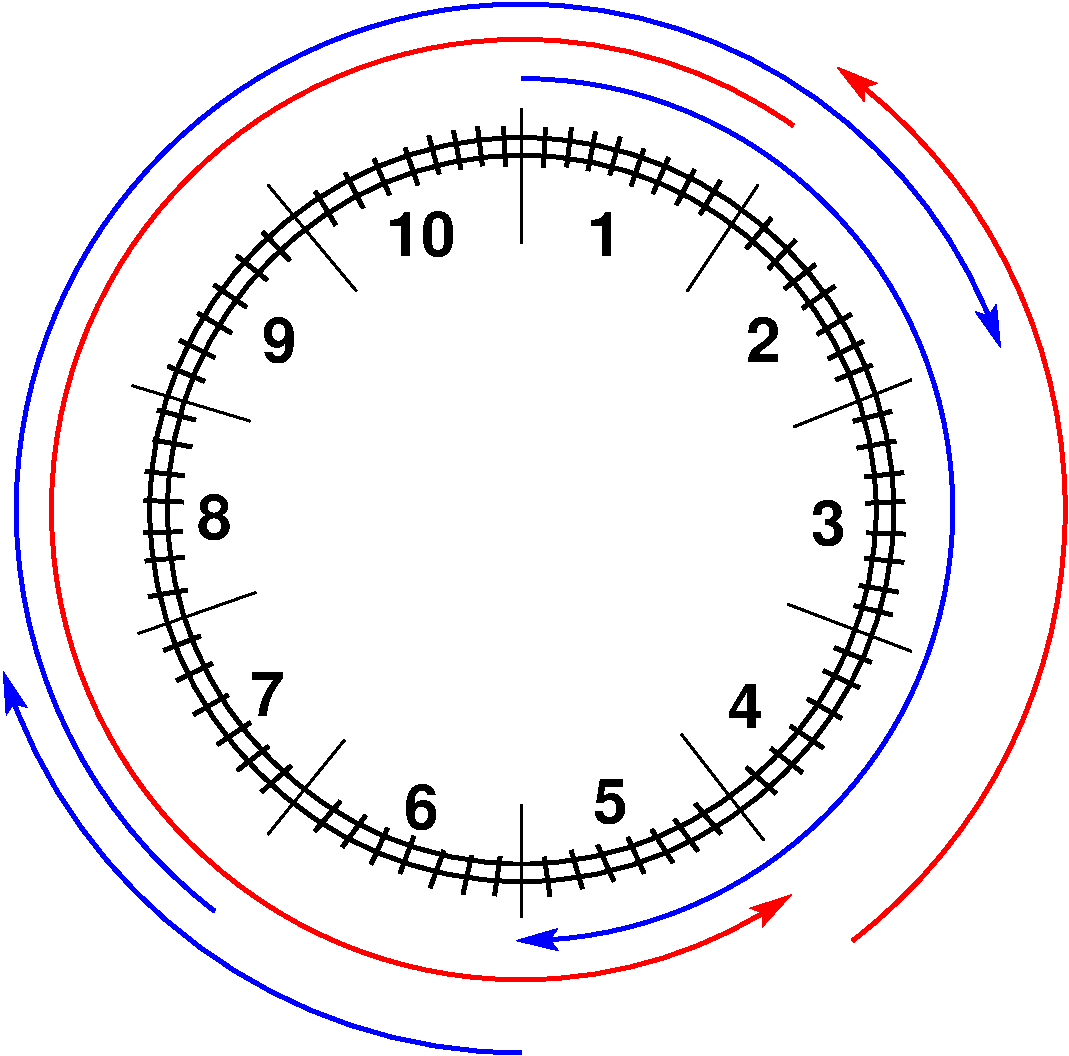
\includegraphics[width=10cm]{alternatingfig.pdf}\\
{\em A possible solution to the first sample. The curved arrows outside the railway represent the arcs that provide electricity. The direction of each arrow represents Fredrik's choice of direction of the electricity (with the blue and red colors emphasizing the different directions). Note that all arrows could have been reversed to get another valid solution: \texttt{11010}.}

\section*{\inputsection}
The first line contains two integers $N$ and $M$.

The next $M$ lines each contain two numbers $1 \le a, b \le N$, indicating that
there is an arc which covers segments $a, a+1, \dots, b$. If $b$ is smaller
than $a$, it means that the sequence wraps around, i.e. segments
$a, \dots, N, 1, \dots, b$ are covered.

\section*{\outputsection}
Print a single line with $M$ \texttt{0}s and \texttt{1}s. The $i$th character of the
line should be \texttt{0} if the $i$th arc given in the input should be oriented
clockwise, or \texttt{1} if it should be oriented counter-clockwise.
If there are multiple solutions you may output any of them.

If it is impossible to orient the arcs, output ``\texttt{impossible}''.

\section*{\constraints}
\testgroups

\noindent
\begin{tabular}{| l | l | l | l |}
\hline
\textbf{\group} & \textbf{\points} & \textbf{\limitsname} & \textbf{\additionalconstraints} \\ \hline
  1     & 20     & $2 \le N, M \le 15$ & \\ \hline
  2     & 20     & $2 \le N, M \le 100$ & \\ \hline
  3     & 20     & $2 \le N, M \le 1000$ & \\ \hline
  4     & 20     & $2 \le N, M \le 10^5$ & no arc has $b < a$ \\ \hline
  5     & 20     & $2 \le N, M \le 10^5$ & \\ \hline
\end{tabular}

% TODO sample description
% Maybe not needed, because the explanation is in the figure caption.
